% Generated by Listas/make_statements.py from pratica-lecture-03.md, item 7. Do not edit.
\textbf{Source.} Muñoz-Garcia \& Toro-Gonzalez (2019), \emph{Strategy and Game Theory: Practice Exercises with Answers}, Ch. 4, Exercise 9 ``Centipede Game'', pp.~176--177 {[}PDF 188--189{]}. Reproduced verbatim (statement only; the book's worked answer follows it). The figure is printed with the book's subgame boxes already drawn. \emph{Note (not in the book):} the text says depositor 1 moves at the 100th stage, but Fig. 4.31 and the book's answer have depositor 2 as the last mover, choosing between \((99, 101)\) and \((100, 100)\); follow the figure.



\begin{quote}

Consider the game tree in Fig. 4.31, representing the so-called ``centipede game'' between depositor 1 and 2. In the first stage, depositor 1 chooses whether to take the money in the saving account, which yields a payoff of \$2 for him and \$0 for the other depositor, or keep the money in the account. If depositor 1 keeps the money in the account, the game continues to stage 2 where depositor 2 can take the money or keep it in the account for one more period. If he takes the money, he receives a payoff of \$3 while depositor 1 receives only \$1. If depositor 2 keeps the money in the account, then it's depositor 1's turn to choose whether to take the money or keep it for one more period. The game continues with depositors alternatively choosing whether to take the money until the 100th stage, when it is depositor 1's turn to move. Since the game tree has 100 branches pointing down, it is often called the ``centipede'' game since the game tree looks like an insect with 100 legs.



\begin{enumerate}

\def\labelenumi{\alph{enumi}.}

\item

  Find the best response of the last mover.

\item

  Anticipating equilibrium behavior in the 100th stage, find the best response of the previous-to-last mover (the depositor acting in stage 99).

\end{enumerate}



\pandocbounded{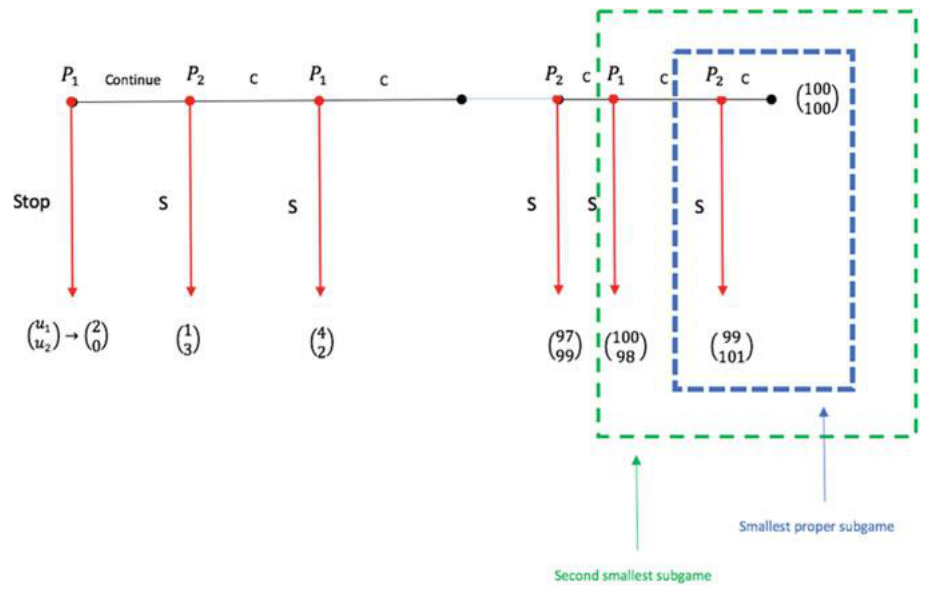
\includegraphics[keepaspectratio,alt={Fig. 4.31 Centipede sequential-form game}]{../figures/munoz-garcia-4-9.png}}



\emph{Fig. 4.31} Centipede sequential-form game



\begin{enumerate}

\def\labelenumi{\alph{enumi}.}

\setcounter{enumi}{2}

\tightlist

\item

  Using your results in parts (a) and (b), find the subgame perfect Nash equilibrium of the game.

\end{enumerate}

\end{quote}



\begin{center}\rule{0.5\linewidth}{0.5pt}\end{center}

